\documentclass[12pt]{article}

% Packages
\usepackage[english]{babel}
\usepackage{caption}
\usepackage[export]{adjustbox}
\usepackage[english]{isodate}
\usepackage[table,svgnames]{xcolor}
\usepackage{url}
\usepackage[utf8x]{inputenc}
\usepackage[T1]{fontenc}
\usepackage{longtable}
\usepackage{amsmath}
\usepackage{graphicx}
\usepackage{parskip}
\usepackage{fancyhdr}
\usepackage{vmargin}
\usepackage{hyperref}
\usepackage[table,svgnames]{xcolor}
\usepackage{longtable}
\usepackage{tabularx}
\usepackage{amsmath}
\usepackage{graphicx}
\usepackage{parskip}
\usepackage{vmargin}
\usepackage{pgfgantt}
\usepackage{pgf-umlcd}
\usepackage{xparse}
\usepackage{float}

\usepackage{tabularx}
\usepackage{titling}
\usepackage{fancyhdr}
% Global graphiscspath
\graphicspath{{../../../img/}}

% Styling changes

%% Better margins
\setmarginsrb{3 cm}{2.5 cm}{3 cm}{2.5 cm}{1 cm}{1.5 cm}{1 cm}{1.5 cm}

\begin{document}


	%%%%%%%%%%%%%%%%%%%%%%%%%%%%%%%%%%%%%%%%%%%%%%%%%%%%%%%%%%%%%%%%%%%%%%%%%%%%%%%%%%%%%%%%% Preface of the report

	% Title Page
	\begin{titlingpage}
		\begin{center}
			\begin{minipage}{\linewidth}
				\centering
				%University logo
				
\includegraphics[width=0.3\linewidth]{FontysLogo.pdf}
				\par
				\vspace{3cm}
				%Thesis title
				{\uppercase
					{\Large Mockups \& Screenshots \\ 2015 Sofa GTL \\ TreeWatch Project
						\par
						\vspace{3cm}}}
				
\includegraphics[width=0.5\linewidth]{TreewatchLogo.pdf}
				\par
				\vspace{2cm}
				%Author's name
				{ Max van der Linden
					\par}
				\vspace{2cm}

				%Date
				\today
			\end{minipage}
		\end{center}
	\end{titlingpage}
	\clearpage

	\section*{Document information}
	\begin{tabular}{ll}
		\textbf{Document name:} & Mockups \& Screenshots\\
		\textbf{Document owner:} & Max van der Linden \\
		\textbf{Company/Organisation:} & Fleuren Baarlo \\
		\textbf{Contact person:} & Max van der Linden, Group leader \\
		\textbf{Date:} & \today \\
		\textbf{Place:} & Fontys University of Applied Science Venlo \\
		\textbf{Authors:} & \parbox[t]{5cm}{
			Max van der Linden\\ max.vanderlinden@student.fontys.nl\\ 2209349 \\ \\}
	\end{tabular}

	\pagebreak

	\tableofcontents
	\clearpage

\section{Mockups \& Screenshot comparisson}
This document contains an overview of the mockups and how they eventually turned out when implemented.
\subsection{Field View}
\begin{figure}[ht]
	\minipage{0.33\textwidth}
	\centering
	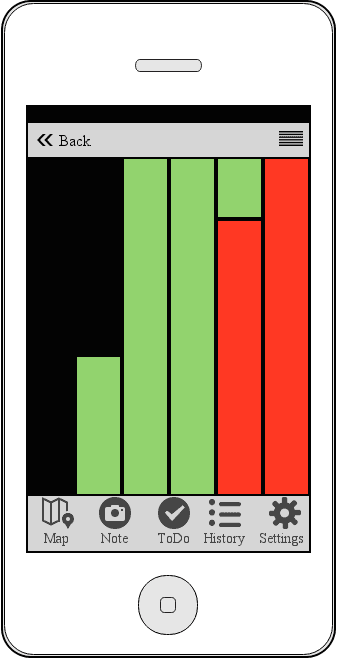
\includegraphics[width=\linewidth, height=0.4\textheight, keepaspectratio=true]{screenshots/Grutto.png}
	\caption{Mockup}
	\endminipage\hfill
	\minipage{0.33\textwidth}
	\centering
	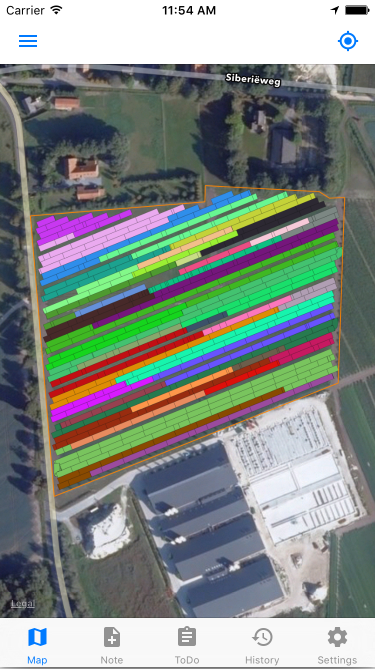
\includegraphics[width=\linewidth, height=0.4\textheight, keepaspectratio=true, frame]{screenshots/GruttoIos.png}
	\caption{IOS}
	\endminipage\hfill
	\minipage{0.33\textwidth}
	\centering
	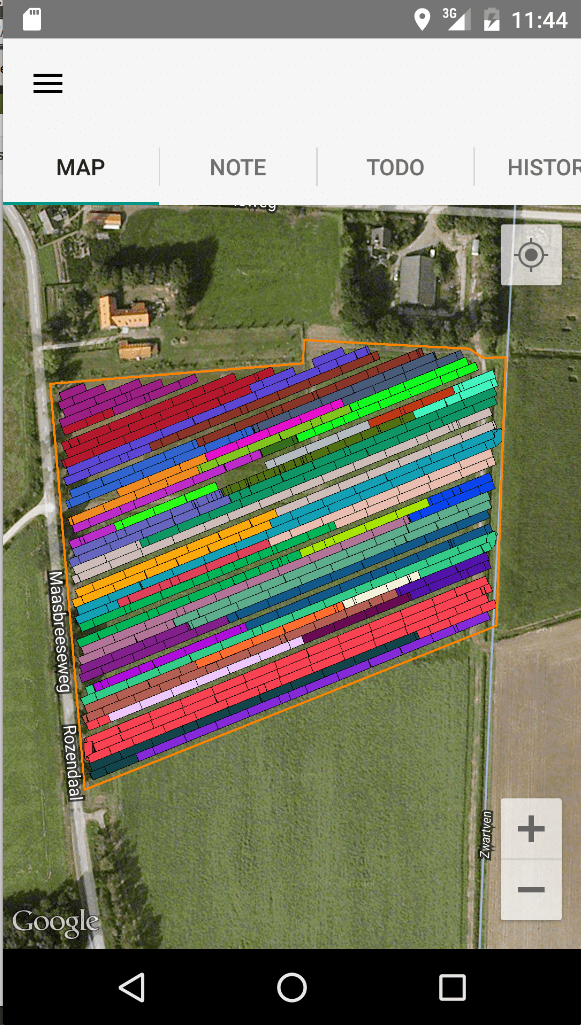
\includegraphics[width=\linewidth, height=0.4\textheight, keepaspectratio=true, frame]{screenshots/GruttoAnd.png}
	\caption{Android}
	\endminipage\hfill
\end{figure}
\clearpage
\subsection{Field Menu}
\begin{figure}[ht]
	\minipage{0.33\textwidth}
	\centering
	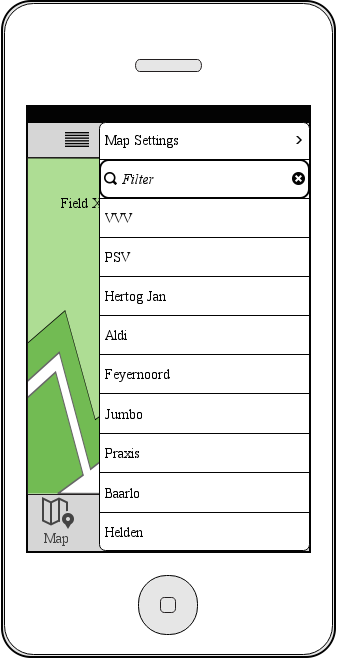
\includegraphics[width=\linewidth, height=0.4\textheight, keepaspectratio=true]{screenshots/Menu.png}
	\caption{Mockup}
	\endminipage\hfill
	\minipage{0.33\textwidth}
	\centering
	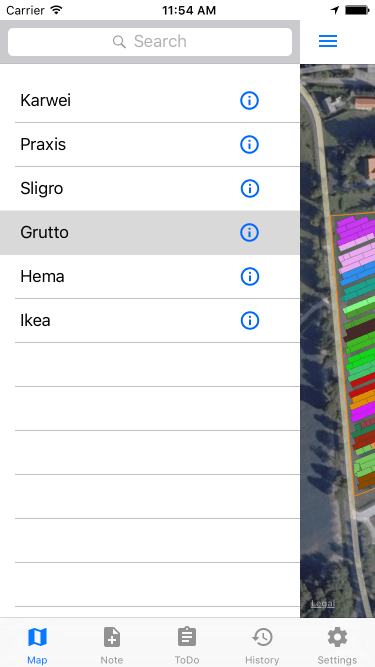
\includegraphics[width=\linewidth, height=0.4\textheight, keepaspectratio=true, frame]{screenshots/MenuIos.png}
	\caption{IOS}
	\endminipage\hfill
	\minipage{0.33\textwidth}
	\centering
	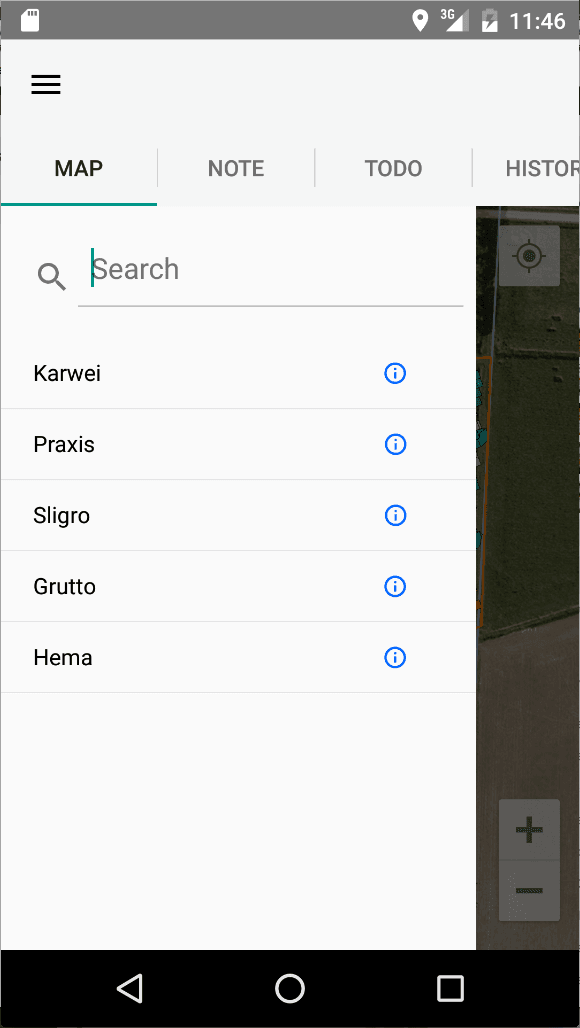
\includegraphics[width=\linewidth, height=0.4\textheight, keepaspectratio=true, frame]{screenshots/MenuAnd.png}
	\caption{Android}
	\endminipage\hfill
\end{figure}
\clearpage
\subsection{Field Info}
\begin{figure}[ht]
	\minipage{0.5\textwidth}
	\centering
	\includegraphics[width=\linewidth, height=0.4\textheight, keepaspectratio=true, frame]{screenshots/RecordsIos.png}
	\caption{IOS}
	\endminipage\hfill
	\minipage{0.5\textwidth}
	\centering
	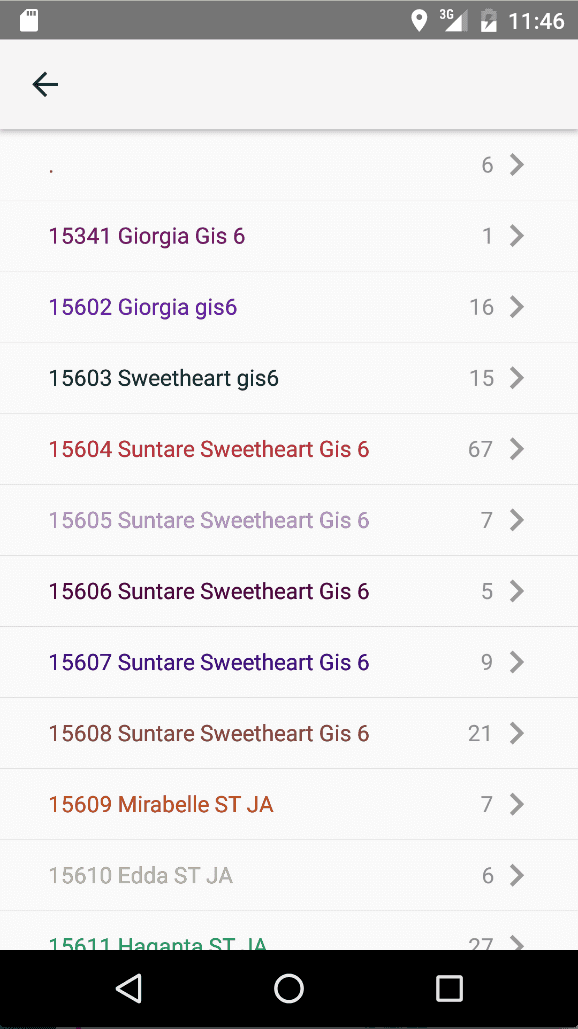
\includegraphics[width=\linewidth, height=0.4\textheight, keepaspectratio=true, frame]{screenshots/RecordsAnd.png}
	\caption{Android}
	\endminipage\hfill
\end{figure}
\clearpage
\subsection{Settings}
\begin{figure}[ht]
	\minipage{0.33\textwidth}
	\centering
	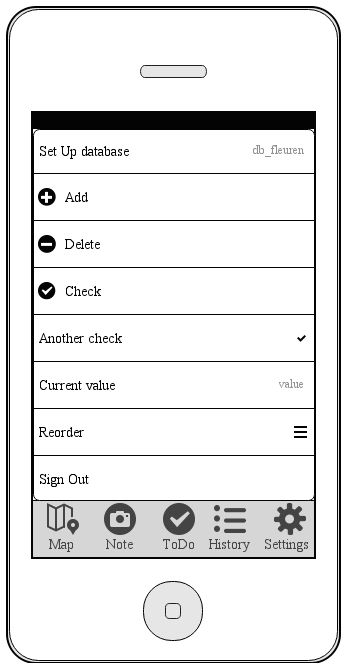
\includegraphics[width=\linewidth, height=0.4\textheight, keepaspectratio=true]{screenshots/Settings.png}
	\caption{Mockup}
	\endminipage\hfill
	\minipage{0.33\textwidth}
	\centering
	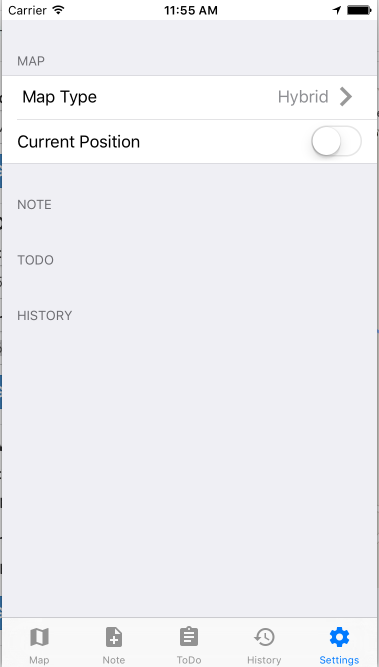
\includegraphics[width=\linewidth, height=0.4\textheight, keepaspectratio=true, frame]{screenshots/SettingsIos.png}
	\caption{IOS}
	\endminipage\hfill
	\minipage{0.33\textwidth}
	\centering
	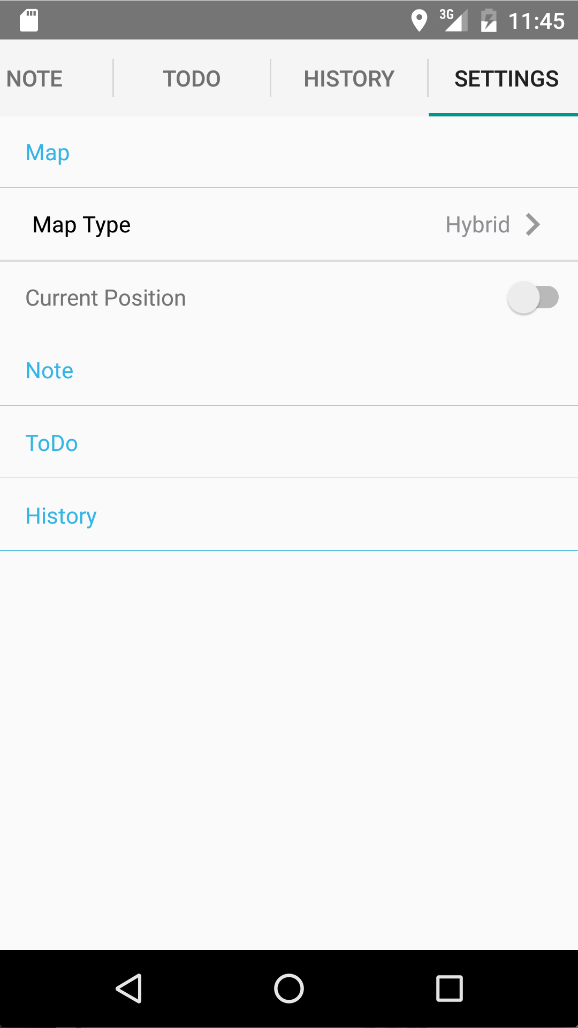
\includegraphics[width=\linewidth, height=0.4\textheight, keepaspectratio=true, frame]{screenshots/SettingsAnd.png}
	\caption{Android}
	\endminipage\hfill
\end{figure}
\clearpage
\subsection{Extra}
\begin{figure}[ht]
	\minipage{0.5\textwidth}
	\centering
	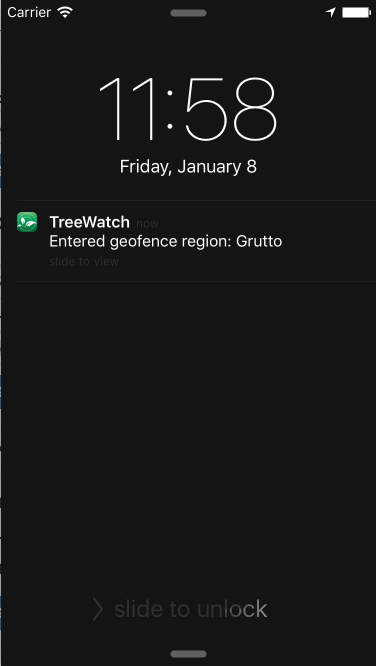
\includegraphics[width=\linewidth, height=0.4\textheight, keepaspectratio=true, frame]{screenshots/GeofenceIos.png}
	\caption{IOS}
	\endminipage\hfill
	\minipage{0.5\textwidth}
	\centering
	
\includegraphics[width=\linewidth, height=0.4\textheight, keepaspectratio=true, frame]{screenshots/LoadAnd.png}
	\caption{Android}
	\endminipage\hfill
\end{figure}
\clearpage
\section{Mockups}
\begin{figure}[ht]
	\minipage{0.33\textwidth}
	\centering
	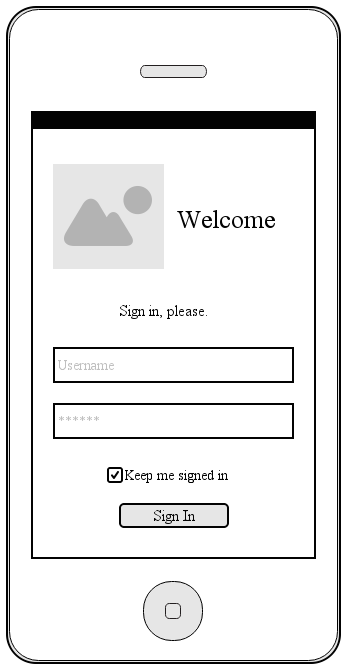
\includegraphics[width=\linewidth, height=0.4\textheight, keepaspectratio=true]{mockups/SignIn.png}
	\caption{Sign In}
	\endminipage\hfill
	\minipage{0.33\textwidth}
	\centering
	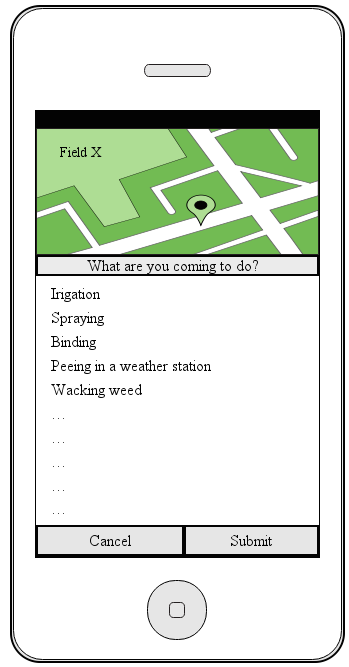
\includegraphics[width=\linewidth, height=0.4\textheight, keepaspectratio=true]{mockups/NotificationComingToDo.png}
	\caption{What are you coming to do?}
	\endminipage\hfill
	\minipage{0.33\textwidth}
	\centering
	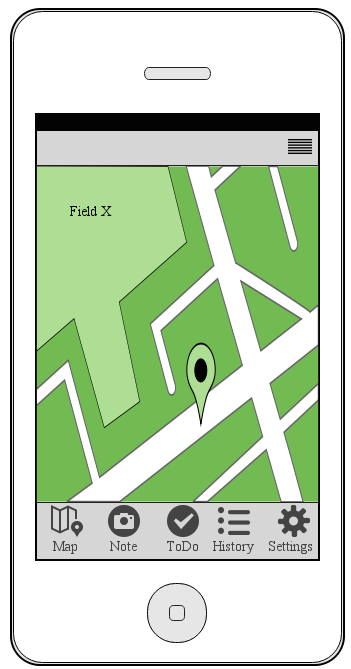
\includegraphics[width=\linewidth, height=0.4\textheight, keepaspectratio=true]{mockups/Map.png}
	\caption{Map}
	\endminipage\hfill
\end{figure}
\begin{figure}[ht]
	\minipage{0.33\textwidth}
	\centering
	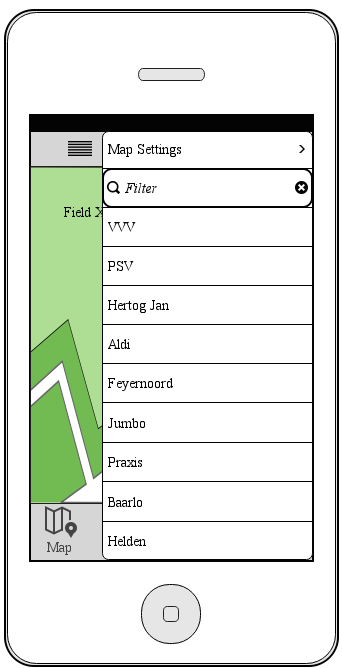
\includegraphics[width=\linewidth, height=0.4\textheight, keepaspectratio=true]{mockups/MapMenu.png}
	\caption{Map Menu}
	\endminipage\hfill
	\minipage{0.33\textwidth}
	\centering
	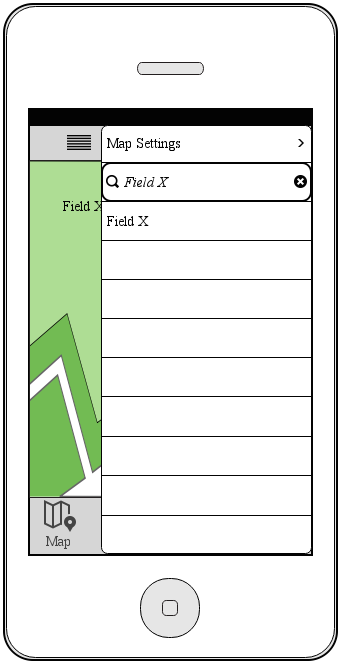
\includegraphics[width=\linewidth, height=0.4\textheight, keepaspectratio=true]{mockups/MapMenuFilter.png}
	\caption{Map menu filter}
	\endminipage\hfill
	\minipage{0.33\textwidth}
	\centering
	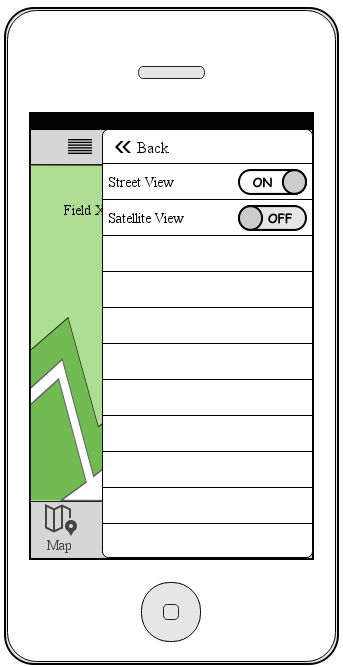
\includegraphics[width=\linewidth, height=0.4\textheight, keepaspectratio=true]{mockups/MapMenuMapSettings.png}
	\caption{Map menu settings}
	\endminipage\hfill
\end{figure}
\begin{figure}[ht]
	\minipage{0.33\textwidth}
	\centering
	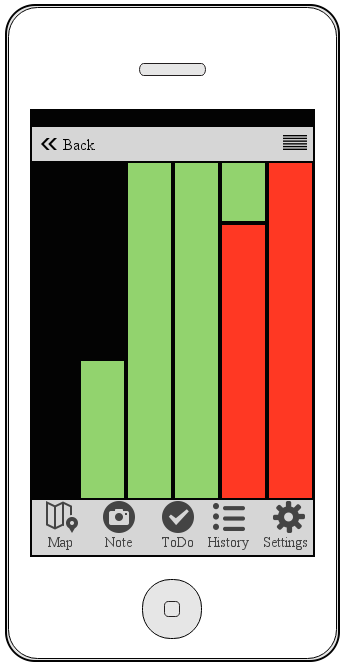
\includegraphics[width=\linewidth, height=0.4\textheight, keepaspectratio=true]{mockups/Overlay.png}
	\caption{Overlay}
	\endminipage\hfill
	\minipage{0.33\textwidth}
	\centering
	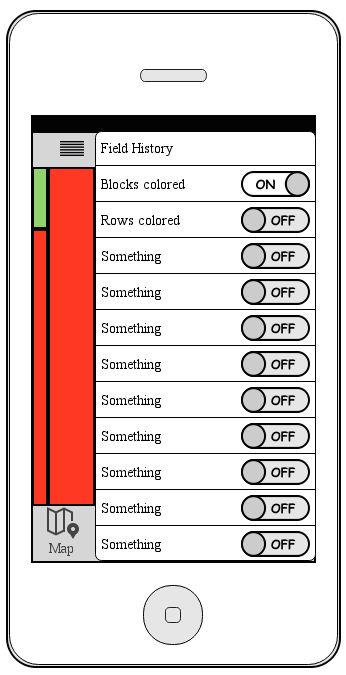
\includegraphics[width=\linewidth, height=0.4\textheight, keepaspectratio=true]{mockups/OverlayMenu.png}
	\caption{Overlay Menu}
	\endminipage\hfill
	\minipage{0.33\textwidth}
	\centering
	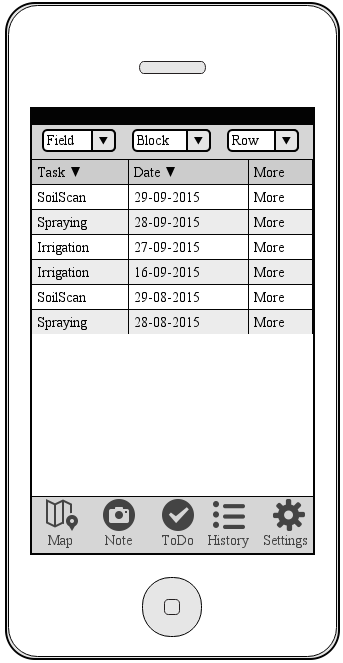
\includegraphics[width=\linewidth, height=0.4\textheight, keepaspectratio=true]{mockups/History.png}
	\caption{History}
	\endminipage\hfill
\end{figure}
\begin{figure}[ht]
	\minipage{0.33\textwidth}
	\centering
	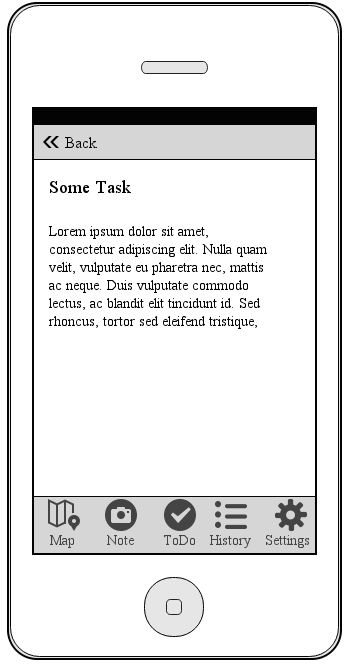
\includegraphics[width=\linewidth, height=0.4\textheight, keepaspectratio=true]{mockups/HistoryMore.png}
	\caption{History More}
	\endminipage\hfill
	\minipage{0.33\textwidth}
	\centering
	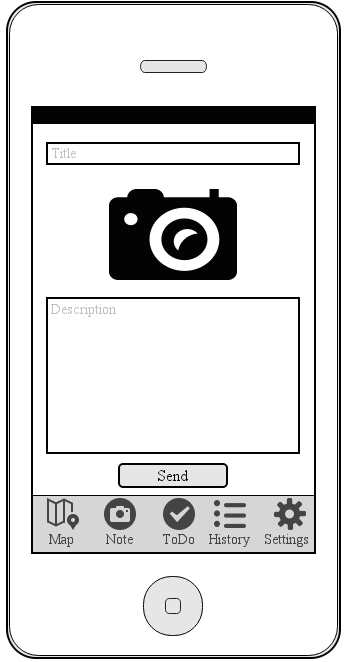
\includegraphics[width=\linewidth, height=0.4\textheight, keepaspectratio=true]{mockups/Note.png}
	\caption{Note}
	\endminipage\hfill
	\minipage{0.33\textwidth}
	\centering
	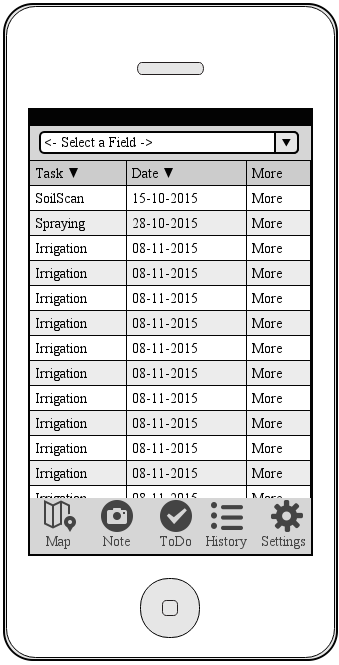
\includegraphics[width=\linewidth, height=0.4\textheight, keepaspectratio=true]{mockups/ToDo.png}
	\caption{}
	\endminipage\hfill
\end{figure}
\begin{figure}[ht]
	\minipage{0.33\textwidth}
	\centering
	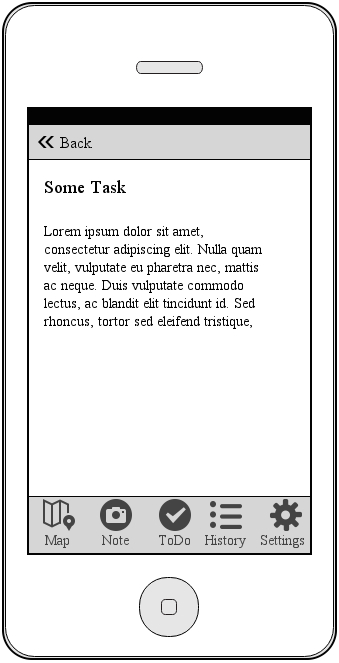
\includegraphics[width=\linewidth, height=0.4\textheight, keepaspectratio=true]{mockups/ToDoMore.png}
	\caption{ToDo More}
	\endminipage\hfill
	\minipage{0.33\textwidth}
	\centering
	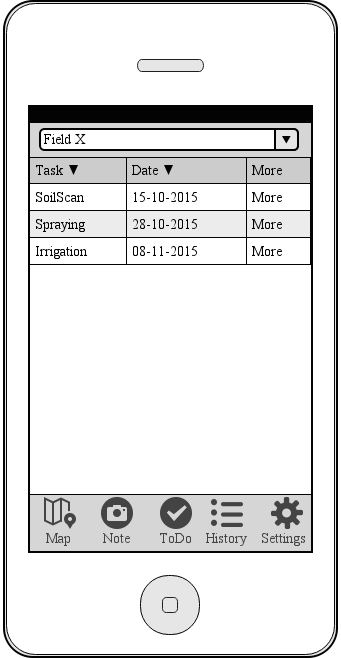
\includegraphics[width=\linewidth, height=0.4\textheight, keepaspectratio=true]{mockups/ToDoFieldX.png}
	\caption{ToDo for Field X}
	\endminipage\hfill
	\minipage{0.33\textwidth}
	\centering
	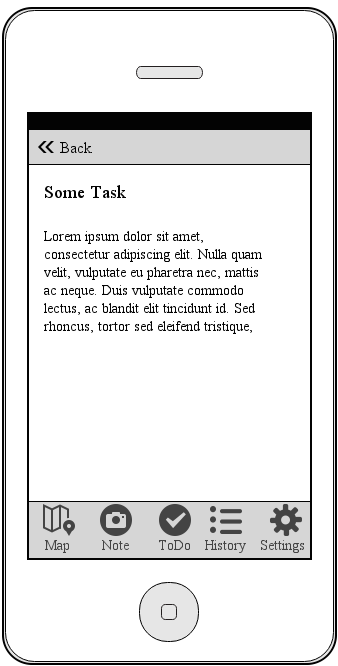
\includegraphics[width=\linewidth, height=0.4\textheight, keepaspectratio=true]{mockups/ToDoFieldXMore.png}
	\caption{ToDo for Field X more}
	\endminipage\hfill
\end{figure}
\begin{figure}[ht]
\minipage{0.33\textwidth}
\centering
\includegraphics[width=\linewidth, height=0.4\textheight, keepaspectratio=true]{mockups/settings.png}
\caption{settings}
\endminipage\hfill
\end{figure}
\end{document}
